
%%%%%%%%%%%%%%%%%%%%%%%%%%%%%%%%%%%%%%%%%%%%%%%%%%%%%%%%%%%
\subsection{Human-swarm interaction results}\label{sec:expResults}
%%%%%%%%%%%%%%%%%%%%%%%%%%%%%%%%%%%%%%%%%%%%%%%%%%%%%%%%%%%

We designed six experiments to investigate human control of large robotic swarms for manipulation tasks.  Screenshots of each experiment are shown in Fig.~\ref{fig:5experiments}.  Each experiment examined the effects of varying a single parameter: population of robots for manipulation, four levels of visual feedback, different levels of Brownian noise, position control with 1 to 10 robots, and three control architectures for both an assembly task and a foraging task. The users could choose which experiment to try, and then our architecture randomly assigned a particular parameter value for each trial.  We recorded the completion time and the participant ID for each successful trial.  
%As Fig.~\ref{fig:Learning} shows, one-third of all participants played only a single game.  Still, many played multiple games, and their decreasing completion times demonstrates their skills improved.


\paragraph{Varying number}
\begin{figure}
\begin{overpic}[width = 0.5\columnwidth]{ResVaryNum.pdf}\end{overpic}
\begin{overpic}[width = 0.48\columnwidth]{measureLearning.pdf}\end{overpic}
\caption{
\label{fig:ResVaryNu}Data from \emph{Varying Number} using robots to push an object through a maze to a goal location.  (Left) Data indicates this task has an optimal number of robots, perhaps due to the relative sizes of the robots, obstacles, and object. Best-fit linear and quadratic lines are overlaid for comparison. 
(Right) Skill improves as players retry tests using data from \emph{Varying Number}.
}
\end{figure}



Transport of goods and materials between points is at the heart of all engineering and construction in real-world systems. This experiment varied from 1 to 500 the population of robots used to transport an object. We kept the total area, maximum robot speed, and total net force the swarm could produce constant. The robots pushed a large hexagonal object through an  {\sffamily S}-shaped maze. Our hypothesis was that participants would complete the task faster with more robots. The results, shown in Fig.~\ref{fig:ResVaryNu}, do not support our hypothesis, indicating rather that there is a local minima around 130 robots.



\paragraph{Varying visualization}

Sensing is expensive, especially on the nanoscale. To see nanocars~\cite{Chiang2011}, scientists fasten molecules that fluoresce light when activated by a strong light source. Unfortunately, multiple exposures can destroy these molecules, a process called \emph{photobleaching}. Photobleaching can be minimized by lowering the excitation light intensity, but \cite{Cazes2001} showed this increases the probability of missed detections.  This experiment explores manipulation with varying amounts of sensing information: {\bf full-state} sensing provides the most information by showing the position of all robots; {\bf convex-hull} draws a convex hull around the outermost robots; {\bf mean} provides the average position of the population; and {\bf mean + variance} adds a confidence ellipse. Fig.~\ref{fig:Visualization} shows screenshots of the same robot swarm with each type of visual feedback. Full-state requires $2n$ data points for $n$ robots. Convex-hull requires at worst $2n$, but usually a smaller number.  Mean requires two, and variance three, data points.  Mean and mean + variance are convenient even with millions of robots. Our hypothesis predicted a steady decay in performance as the amount of visual feedback decreased.

%\begin{figure}[b!]
%\renewcommand{\figwid}{0.5\columnwidth}
%\begin{overpic}[width =\figwid]{ResVaryVis.pdf}\end{overpic}
%\vspace{-1em}
%\caption{\label{fig:ResVaryVis} Completion-time results for the four levels of visual feedback shown in Fig.~\ref{fig:Visualization}.  Players performed better with limited feedback.
%%\vspace{-1em}
%}
%\end{figure}

\begin{wrapfigure}{R}{0.5\textwidth}
  \vspace{-20pt}
  \begin{center}
  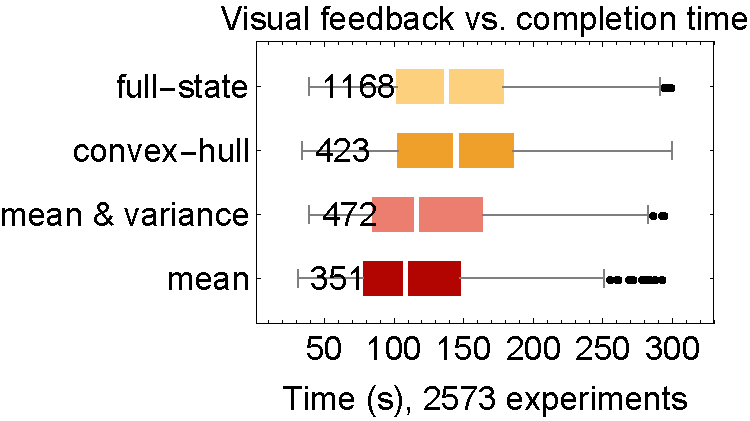
\includegraphics[width=0.5\textwidth]{ResVaryVis.pdf}
  \end{center}
  \vspace{-1em}
\caption{\label{fig:ResVaryVis} Completion-time results for the four levels of visual feedback shown in Fig.~\ref{fig:Visualization}.  Players performed better with limited feedback.
\vspace{-1em}
}
\end{wrapfigure}


% Additionally, as population characteristics, they are available even if only a percentage of the robots are detected each control cycle.
%Photobleaching: http://www.piercenet.com/browse.cfm?fldID=4DD9D52E-5056-8A76-4E6E-E217FAD0D86B
%
%Photobleaching is caused by the irreversible destruction of fluorophores due to either the prolonged exposure to the excitation source or exposure to high-intensity excitation light. Photobleaching can be minimized or avoided by exposing the fluor(s) to the lowest possible level of excitation light intensity for the shortest length of time that still yields the best signal detection; this requires optimization of the detection method using high sensitivity CCD cameras, high numerical aperture objective and/or the widest bandpass emission filter(s) available. Other approaches include using fluorophores that are more photostable than traditional fluorophores and/or using antifade reagents to protect the fluor(s) against photobleaching. Steps to avoid photobleaching are not feasible for all detection methods and should be optimized for each method used. For example, antifade reagents are toxic to live cells, and therefore they can only be used with fixed cells or tissue. Furthermore, some detection methods, such as flow cytometry, normally do not require steps to avoid photobleaching because of the extremely short exposure time of the fluorophore to the excitation source.


%\begin{figure}
%\centering
%\begin{overpic}[width = \columnwidth]{ResVaryVis.pdf}\end{overpic}
%\vspace{-2em}
%\caption{\label{fig:ResVaryVis} Completion-time results for the four levels of visual feedback shown in Fig.~\ref{fig:Visualization}. Surprisingly, players perform better with limited feedback--subjects with only the mean + variance  outperformed all others.
%\vspace{-2em}
%}
%\end{figure}

\begin{figure}[b!]
\renewcommand{\figwid}{0.24\columnwidth}
\begin{overpic}[width =\figwid]{VaryVisFS.pdf}\put(20,15){Full-state}\end{overpic}
\begin{overpic}[width =\figwid]{VaryVisCH.pdf}\put(10,15){Convex-hull}\end{overpic}
\begin{overpic}[width =\figwid]{VaryVisMV.pdf}\put(10,15){Mean + var}\end{overpic}
\begin{overpic}[width =\figwid]{VaryVisMe.pdf}\put(30,15){Mean}\end{overpic}
\vspace{-.5em}
\caption{\label{fig:Visualization}Screenshots from task \emph{Vary Visualization}. This experiment challenges players to quickly steer 100 robots (blue discs) to push an object (green hexagon) into a goal region. We record the completion time and other statistics.
%\vspace{-1em}
}
\end{figure}

Our experiment indicated the opposite: players with just the mean completed the task faster than those with full-state feedback.  As Fig.~\ref{fig:ResVaryVis}.b shows, the levels of feedback arranged by increasing completion time are [mean + variance, mean, full-state, convex-hull].  All experiments lasting over 300s were removed, under the assumption that the user stopped playing
Using ANOVA analysis, we reject the null hypothesis that all visualization methods are equivalent, with $p$-value $2.69\times10^{-19}$.
Anecdotal evidence from beta-testers who played the game suggests that tracking 100 robots is overwhelming---similar to schooling phenomenons that confuse predators---while working with just the mean + variance is like using a ``spongy'' manipulator. Our beta-testers found convex-hull feedback confusing and irritating.  A single robot left behind an obstacle will stretch the entire hull, obscuring the majority of the swarm.
%obscuring what the rest of the swarm is doing.   

\paragraph{Varying noise}
Microrobots are affected by turbulence caused by random collisions with molecules. The effect of these collisions is called Brownian motion.

This experiment varied the strength of these disturbances to study how noise affects human control of large swarms. Noise was applied at every timestep as follows:
\begin{align*}
\dot{x}_i &= u_x + m_i\cos(\psi_i)\\
 \dot{y}_i &= u_y + m_i\sin(\psi_i).
 \end{align*}
$m_i,\psi_i$ are uniformly IID, with $m_i\in[0,M]$ and $\psi_i\in[0,2\pi]$. $M$ is a constant for each trial ranging from 0 to 200\% of the maximum control power ($u_{max}$).
 
We hypothesized 200\% noise was the largest a human could be expected to control---at 200\% noise, the robots move erratically.  Disproving our hypothesis, the results in Fig.~\ref{fig:ResVaryNoisePosition}.a show only a 40\% increase in completion time for the maximum noise.

\begin{figure}[b!]
\renewcommand{\figwid}{0.5\columnwidth}
\begin{overpic}[width =\figwid]{ResVaryNoise.pdf}\end{overpic}
\begin{overpic}[width =\figwid]{ResPositioning.pdf}\end{overpic}
\vspace{-1em}
\caption{\label{fig:ResVaryNoisePosition} Left: Varying the noise from 0 to 200\% of the maximum control input resulted in only a small increase in completion time. Right: Increasing the number of robots resulted in longer completion times.  For more than 4 robots the goal pattern contained a void, which may have caused the longer completion times.
%\vspace{-1em}
}
\end{figure}


\paragraph{Position control}
This online experiment examined how completion time scales with the number of robots $n$. Using a single square obstacle, users arranged $n\in[1,10]$ robots into a specified goal pattern.  The goal pattern formed a block  {\sffamily A} with 10 robots, and lesser numbers of robots used a subset of these goal positions. Our hypothesis was that completion time would increase linearly with the number of robots, as with our position control algorithm in \cite{Becker2013b}.  Our results roughly corroborate this, as shown in Fig.~\ref{fig:ResVaryNoisePosition}.b.  Though the number of robots presented to game players is uniformly distributed, larger $n$ are more difficult, and the number of successful experiments drops steadily as $n$ increases.



Note there is a bifurcation between $n$=4 and $n$=5 robots. For $n\in[1,4]$ the goal patterns are not hollow, but starting at $n$=5 they are.  A better experiment design would randomly place the goal positions.  Initially we tried this, but our beta-testers strongly disliked trying to arrange robots in random patterns.


\paragraph{Varying control: Assembly}
Ultimately, we want to use swarms of robots to build things. This experiment compared different control architectures modeled after real-world devices.

We compared attractive and repulsive control with the global control used for the other experiments. The attractive and repulsive controllers were loosely modeled after scanning tunneling microscopes (STM), but also apply to magnetic manipulation, e.g.\ \cite{Khalil2013} and biological models, e.g. \cite{goodrich2012types}. STMs can be used to arrange atoms and make small assemblies~\cite{avouris1995manipulation}. An STM tip is charged with electrical potential, and used to repel like-charged or to attract differently-charged molecules. In contrast, the global controller uses a uniform field (perhaps formed by parallel lines of differently-charged conductors) to pull molecules in the same direction.
The experiment challenged players to assemble a three-block pyramid with a swarm of 16 robots.

%\todo{describe controller model here, use an equation}

The results were conclusive, as shown in Fig.~\ref{fig:ResVaryControl}.a: attractive control was the fastest, followed by global control, with repulsive control a distant last.  The median time using repulsive control was four times longer than with attractive control.
Using ANOVA analysis, we reject the null hypothesis that all controllers are equivalent, with $p$-value $3.37\times10^{-32}$.

%%\begin{figure}
%%\begin{overpic}[width = 0.39\columnwidth]{attractiveForce.pdf}\end{overpic}
%%\begin{overpic}[width = 0.6\columnwidth]{understandingForces.pdf}\end{overpic}
%%\caption{
%%\label{fig:attractiveForce}
%%Attraction and repulsion with a point source distance $h$ above the plane and $r$ from the robot. 
%%}
%%\end{figure}

\begin{figure}[b!]
\renewcommand{\figwid}{3.3cm}
\begin{overpic}[height =\figwid]{ResVaryControl.pdf}\end{overpic}
\begin{overpic}[height =\figwid]{ResVaryForage.pdf}\end{overpic}
\vspace{-.5em}
\caption{\label{fig:ResVaryControl} Completion time depends on both the task and the control type. Left: Attractive control resulted in the shortest completion time and repulsive the longest for building a three-block pyramid. Right: in the foraging test, global control resulted in the shortest completion time and attractive the longest.
%\vspace{-1em}
}
\end{figure}

\paragraph{Varying control: Foraging}
Collecting and delivering resources is necessary for drug delivery.
This experiment also compared attractive and repulsive control with the global control used for the other experiments. The experiment challenged players to collect particles using a swarm of 100 robots and return the particles to a home region. The robots encapsulate the particles on contact. 

%\todo{describe controller model here, use an equation}

The results were conclusive, as shown in Fig.~\ref{fig:ResVaryControl}.b: global control was the fastest, followed by repulsive control, with attractive control last.  Using ANOVA analysis, we reject the null hypothesis that all controllers are equivalent, with $p$-value $2.96\times10^{-6}$.


